\documentclass[11pt,twocolumn]{article}

\usepackage[margin=1in]{geometry}
\usepackage{amsmath,amssymb,amsfonts}
\usepackage{tikz}
\usepackage{pgfplots}
\pgfplotsset{compat=1.18}
\usepackage{booktabs}
\usepackage{hyperref}
\usepackage{xcolor}
\usepackage{listings}
\usepackage{algorithm}
\usepackage{algorithmic}

\definecolor{alive}{HTML}{2D7D46}
\definecolor{dead}{HTML}{E8E8E8}
\definecolor{convblue}{HTML}{3366CC}
\definecolor{relured}{HTML}{CC3333}

\lstset{
  basicstyle=\ttfamily\footnotesize,
  keywordstyle=\color{convblue}\bfseries,
  commentstyle=\color{gray},
  numbers=left,
  numberstyle=\tiny\color{gray},
  breaklines=true,
  frame=single,
  framesep=3pt,
  xleftmargin=1.5em,
}

\title{One Primitive: Running Conway's Game of Life\\and a Transformer on Apple's Neural Engine\\via Convolution}

\author{Alvaro Videla\\
\textit{Microsoft}}

\date{April 2026}

\begin{document}
\maketitle

\begin{abstract}
We show that a single operation---convolution---suffices to run both
Conway's Game of Life (GOL) and a full transformer language model on
Apple's Neural Engine (ANE).
%
GOL is encoded as a 3$\times$3 convolution with ReLU-based rule
evaluation, achieving 2.3~billion cell-generations per second on a
1024$\times$1024 grid (2.5$\times$ faster than CPU).
%
The Qwen2.5-0.5B transformer is mapped entirely to
\texttt{Conv2d(1$\times$1)} operations, with every linear projection
expressed as a 1$\times$1 convolution, achieving 90~tokens/sec decode
throughput---within 4$\times$ of llama.cpp on Metal GPU, using a
compute unit (ANE) that conventional LLM engines ignore.
%
Both systems share the same silicon: the ANE's 16-core convolution
engine. We describe the algebraic encoding of GOL rules into
convolution + ReLU, the transformer-to-convolution mapping, and a
series of book-driven optimizations that improved decode throughput by
10$\times$ from initial implementation to final system.
\end{abstract}

%% ════════════════════════════════════════════════════════════════════
\section{Introduction}
\label{sec:intro}

Apple's Neural Engine (ANE), present in every Apple Silicon chip since
A11, is a hardware accelerator optimized for convolution, element-wise
arithmetic, and activation functions. Unlike the GPU---which excels at
arbitrary parallel kernels---the ANE achieves peak throughput on a
narrow set of operations: small-kernel convolutions, ReLU, and
channel-wise reductions.

This paper demonstrates that convolution alone is a sufficient
primitive to implement two seemingly different computations on the ANE:

\begin{enumerate}
\item \textbf{Conway's Game of Life} --- a cellular automaton where
each generation is a 3$\times$3 convolution counting neighbors,
followed by ReLU-based rule evaluation.

\item \textbf{Transformer inference} --- a Qwen2.5-0.5B language model
where every matrix multiplication is expressed as a
\texttt{Conv2d(1$\times$1)} operation.
\end{enumerate}

The connection is not metaphorical. Both computations compile to the
same ANE instruction stream: convolution kernels dispatched to the
same 16-core engine. The key insight is that the ANE's convolution
unit can execute any linear operation when the spatial dimensions are
1$\times$1 (reducing to matrix--vector multiply) and any local
cellular rule when the spatial dimensions match the grid.

Section~\ref{sec:gol} presents the GOL encoding.
Section~\ref{sec:transformer} describes the transformer mapping.
Section~\ref{sec:opt} details the optimization journey.
Section~\ref{sec:results} presents benchmarks.
Section~\ref{sec:related} discusses related work.

%% ════════════════════════════════════════════════════════════════════
\section{Game of Life as Convolution}
\label{sec:gol}

\subsection{The Encoding}

Conway's Game of Life operates on a binary grid where each cell is
alive (1) or dead (0). The rules depend on the count of alive
neighbors (out of 8):

\begin{itemize}
\item \textbf{Birth}: A dead cell with exactly 3 neighbors becomes alive.
\item \textbf{Survival}: An alive cell with 2 or 3 neighbors stays alive.
\item \textbf{Death}: All other cells die (or remain dead).
\end{itemize}

We encode one GOL generation as a convolution followed by ReLU-based
rule evaluation.

\paragraph{Step 1: Convolution.} Apply a 3$\times$3 kernel:
\begin{equation}
K = \begin{bmatrix} 1 & 1 & 1 \\ 1 & 9 & 1 \\ 1 & 1 & 1 \end{bmatrix}
\label{eq:kernel}
\end{equation}

The center weight 9 (rather than 0 or 1) encodes the cell's own state
into the output. For a cell at position $(r,c)$ with value $x_{r,c}
\in \{0,1\}$ and neighbor count $n$:
\begin{equation}
s = n + 9 \cdot x_{r,c} =
\begin{cases}
n       & \text{if dead}   \quad (s \in [0,8]) \\
n + 9   & \text{if alive}  \quad (s \in [9,17])
\end{cases}
\end{equation}

This separates the dead and alive cases into non-overlapping integer
ranges, enabling branchless rule evaluation.

\paragraph{Step 2: ReLU rule evaluation.} We implement an exact
equality test using ReLU:
\begin{equation}
\mathrm{eq}(s, k) = \mathrm{relu}\!\big(1 - (\mathrm{relu}(s-k) + \mathrm{relu}(k-s))\big)
\label{eq:relu_eq}
\end{equation}

This yields exactly 1 when $s = k$ and 0 otherwise (for non-negative
integers). The GOL rules become:
\begin{equation}
x'_{r,c} = \mathrm{clamp}\!\big(\mathrm{eq}(s, 3) + \mathrm{eq}(s, 11) + \mathrm{eq}(s, 12),\; 0,\; 1\big)
\label{eq:gol_rule}
\end{equation}

where $s=3$ captures birth (dead, 3 neighbors), $s=11$ captures
survival with 2 neighbors (alive, $2+9$), and $s=12$ captures
survival with 3 neighbors (alive, $3+9$).

\paragraph{Multi-generation pipelining.} Stacking $N$ copies of the
conv+rule layer produces a single network that computes $N$
generations in one forward pass, pipelined through the ANE's 16 cores.

\subsection{Visual Example}

Figure~\ref{fig:gol_blinker} shows the blinker oscillator (period 2)
through one generation of the convolution encoding.

\begin{figure}[t]
\centering
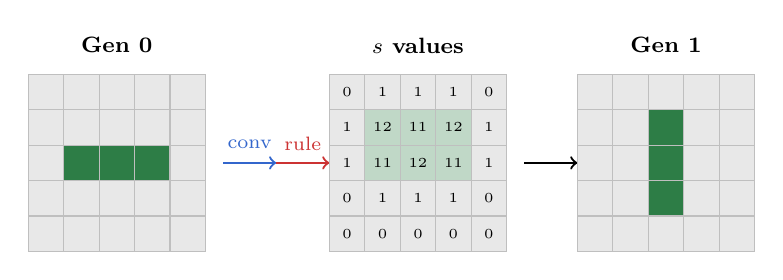
\begin{tikzpicture}[scale=0.45, every node/.style={minimum size=0.45cm, inner sep=0pt}]
% === Generation 0: horizontal blinker ===
\node[anchor=south] at (2.5, 5.3) {\footnotesize\textbf{Gen 0}};
\foreach \r in {0,...,4} {
  \foreach \c in {0,...,4} {
    \fill[dead] (\c, 4-\r) rectangle ++(1,1);
    \draw[gray!50] (\c, 4-\r) rectangle ++(1,1);
  }
}
% Alive cells: row 2, cols 1-3
\fill[alive] (1, 2) rectangle ++(1,1);
\fill[alive] (2, 2) rectangle ++(1,1);
\fill[alive] (3, 2) rectangle ++(1,1);
\draw[gray!50] (1,2) rectangle ++(1,1);
\draw[gray!50] (2,2) rectangle ++(1,1);
\draw[gray!50] (3,2) rectangle ++(1,1);

% Arrow
\draw[->, thick, convblue] (5.5, 2.5) -- (7, 2.5)
  node[midway, above, font=\scriptsize] {conv};
\draw[->, thick, relured] (7, 2.5) -- (8.5, 2.5)
  node[midway, above, font=\scriptsize] {rule};

% === S values (after conv) ===
\node[anchor=south] at (11, 5.3) {\footnotesize\textbf{$s$ values}};
\foreach \r/\vals in {0/{0,1,1,1,0}, 1/{1,12,11,12,1}, 2/{1,11,12,11,1}, 3/{0,1,1,1,0}, 4/{0,0,0,0,0}} {
  \foreach \c [count=\ci from 0] in \vals {
    \pgfmathparse{int(\c)}
    \ifnum\pgfmathresult>8
      \fill[alive!30] (8.5+\ci, 4-\r) rectangle ++(1,1);
    \else
      \fill[dead] (8.5+\ci, 4-\r) rectangle ++(1,1);
    \fi
    \draw[gray!50] (8.5+\ci, 4-\r) rectangle ++(1,1);
    \node[font=\tiny] at (9+\ci, 4.5-\r) {\c};
  }
}

% Arrow
\draw[->, thick] (14, 2.5) -- (15.5, 2.5);

% === Generation 1: vertical blinker ===
\node[anchor=south] at (18, 5.3) {\footnotesize\textbf{Gen 1}};
\foreach \r in {0,...,4} {
  \foreach \c in {0,...,4} {
    \fill[dead] (15.5+\c, 4-\r) rectangle ++(1,1);
    \draw[gray!50] (15.5+\c, 4-\r) rectangle ++(1,1);
  }
}
% Alive cells: col 2, rows 1-3
\fill[alive] (17.5, 3) rectangle ++(1,1);
\fill[alive] (17.5, 2) rectangle ++(1,1);
\fill[alive] (17.5, 1) rectangle ++(1,1);
\draw[gray!50] (17.5,3) rectangle ++(1,1);
\draw[gray!50] (17.5,2) rectangle ++(1,1);
\draw[gray!50] (17.5,1) rectangle ++(1,1);
\end{tikzpicture}
\caption{Blinker oscillator through one GOL generation. Left: the
horizontal blinker (3 alive cells). Center: $s$ values after the
3$\times$3 convolution with kernel $K$. Values $\geq 9$ (shaded)
indicate alive cells. Only positions with $s \in \{3, 11, 12\}$
survive the ReLU rule. Right: the vertical blinker.}
\label{fig:gol_blinker}
\end{figure}

\begin{figure}[t]
\centering
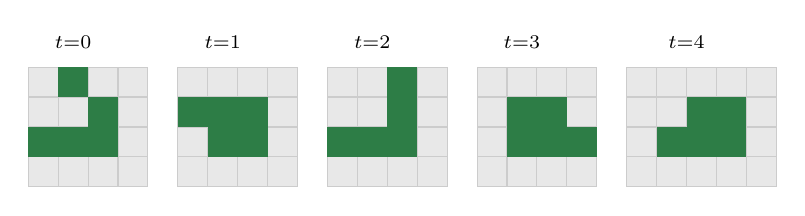
\begin{tikzpicture}[scale=0.38, every node/.style={minimum size=0.38cm, inner sep=0pt}]
% === Glider: 5 generations ===
% Gen 0
\node[anchor=south, font=\scriptsize\bfseries] at (1.5, 4.3) {$t{=}0$};
\foreach \r in {0,...,3} {
  \foreach \c in {0,...,3} {
    \fill[dead] (\c, 3-\r) rectangle ++(1,1);
    \draw[gray!40] (\c, 3-\r) rectangle ++(1,1);
  }
}
\fill[alive] (1,3) rectangle ++(1,1); % (0,1)
\fill[alive] (2,2) rectangle ++(1,1); % (1,2)
\fill[alive] (0,1) rectangle ++(1,1); % (2,0)
\fill[alive] (1,1) rectangle ++(1,1); % (2,1)
\fill[alive] (2,1) rectangle ++(1,1); % (2,2)

% Gen 1
\begin{scope}[xshift=5cm]
\node[anchor=south, font=\scriptsize\bfseries] at (1.5, 4.3) {$t{=}1$};
\foreach \r in {0,...,3} {
  \foreach \c in {0,...,3} {
    \fill[dead] (\c, 3-\r) rectangle ++(1,1);
    \draw[gray!40] (\c, 3-\r) rectangle ++(1,1);
  }
}
\fill[alive] (0,2) rectangle ++(1,1); % (1,0)
\fill[alive] (2,2) rectangle ++(1,1); % (1,2)
\fill[alive] (1,1) rectangle ++(1,1); % (2,1)
\fill[alive] (2,1) rectangle ++(1,1); % (2,2)
\fill[alive] (1,2) rectangle ++(1,1); % (1,1)
\end{scope}

% Gen 2
\begin{scope}[xshift=10cm]
\node[anchor=south, font=\scriptsize\bfseries] at (1.5, 4.3) {$t{=}2$};
\foreach \r in {0,...,3} {
  \foreach \c in {0,...,3} {
    \fill[dead] (\c, 3-\r) rectangle ++(1,1);
    \draw[gray!40] (\c, 3-\r) rectangle ++(1,1);
  }
}
\fill[alive] (2,2) rectangle ++(1,1);
\fill[alive] (1,1) rectangle ++(1,1);
\fill[alive] (2,1) rectangle ++(1,1);
\fill[alive] (0,1) rectangle ++(1,1);
\fill[alive] (2,3) rectangle ++(1,1);
\end{scope}

% Gen 3
\begin{scope}[xshift=15cm]
\node[anchor=south, font=\scriptsize\bfseries] at (1.5, 4.3) {$t{=}3$};
\foreach \r in {0,...,3} {
  \foreach \c in {0,...,3} {
    \fill[dead] (\c, 3-\r) rectangle ++(1,1);
    \draw[gray!40] (\c, 3-\r) rectangle ++(1,1);
  }
}
\fill[alive] (1,2) rectangle ++(1,1);
\fill[alive] (2,1) rectangle ++(1,1);
\fill[alive] (3,1) rectangle ++(1,1);
\fill[alive] (2,2) rectangle ++(1,1);
\fill[alive] (1,1) rectangle ++(1,1);
\end{scope}

% Gen 4
\begin{scope}[xshift=20cm]
\node[anchor=south, font=\scriptsize\bfseries] at (2, 4.3) {$t{=}4$};
\foreach \r in {0,...,3} {
  \foreach \c in {0,...,4} {
    \fill[dead] (\c, 3-\r) rectangle ++(1,1);
    \draw[gray!40] (\c, 3-\r) rectangle ++(1,1);
  }
}
\fill[alive] (2,2) rectangle ++(1,1);
\fill[alive] (3,1) rectangle ++(1,1);
\fill[alive] (1,1) rectangle ++(1,1);
\fill[alive] (2,1) rectangle ++(1,1);
\fill[alive] (3,2) rectangle ++(1,1);
\end{scope}

\end{tikzpicture}
\caption{The glider spaceship translating diagonally over 4
generations, each computed by one conv+ReLU layer on ANE. After 4
generations the pattern has moved one cell down and one cell right.}
\label{fig:gol_glider}
\end{figure}


%% ════════════════════════════════════════════════════════════════════
\section{Transformer as Convolution}
\label{sec:transformer}

\subsection{The Mapping}

The ANE's convolution engine computes $\texttt{Conv2d}(C_\text{in},
C_\text{out}, k_h \times k_w)$. When $k_h = k_w = 1$ and the spatial
dimensions are $1 \times 1$, the operation reduces to:

\begin{equation}
y_i = \sum_{j=1}^{C_\text{in}} W_{ij} \cdot x_j \quad \text{for } i = 1, \ldots, C_\text{out}
\end{equation}

This is a matrix--vector product. Every linear layer in a transformer
can therefore be expressed as \texttt{Conv2d(1$\times$1)} by reshaping
the input to $(B, C, 1, 1)$ format.

\subsection{Qwen2.5-0.5B Architecture}

We target Qwen2.5-0.5B-Instruct (24 layers, $d=896$, 14 attention
heads, 2 KV heads via Grouped Query Attention). The complete mapping:

\begin{center}
\footnotesize
\begin{tabular}{lll}
\toprule
\textbf{Layer} & \textbf{Transformer} & \textbf{Conv2d} \\
\midrule
QKV proj. & $896 \to 1152$ & \texttt{Conv(896, 1152, 1)} \\
Output proj. & $896 \to 896$ & \texttt{Conv(896, 896, 1)} \\
Gate+Up & $896 \to 9728$ & \texttt{Conv(896, 9728, 1)} \\
Down proj. & $4864 \to 896$ & \texttt{Conv(4864, 896, 1)} \\
LM head & $896 \to 151936$ & \texttt{Conv(896, 151936, 1)} \\
\bottomrule
\end{tabular}
\end{center}

RMSNorm, RoPE, softmax, SiLU, and element-wise operations are
expressed as MIL (Model Intermediate Language) primitives that CoreML
maps to the ANE's element-wise ALUs.

\subsection{Grouped Query Attention}

Qwen2.5-0.5B uses 14 query heads with 2 KV groups (7 query heads per
group). A na\"ive implementation requires $14 \times 2 = 28$ separate
matmul+softmax operations per layer, totaling 672 across all 24
layers.

Our batched GQA optimization groups all 7 query heads sharing a KV
group into a single batched matmul:

\begin{equation}
\text{Attn}_g = \text{softmax}\!\left(\frac{Q_g \cdot K_g^T}{\sqrt{d_h}}\right) V_g
\end{equation}

where $Q_g \in \mathbb{R}^{7 \times \text{seq} \times d_h}$ batches
all 7 query heads in group $g$. This reduces the total number of
attention matmul operations from 672 to 96 (a 7$\times$ reduction),
saving approximately 170 MIL operations in the compiled model.

\subsection{Quantization}

Weights are quantized to int8 using block-wise quantization (block
size 32), reducing the model from 942~MB (fp16) to 472~MB. We
evaluated int4 quantization (265~MB) but found it \emph{slower} on
ANE---the hardware has native int8 datapaths but must dequantize int4
at inference time, adding $\sim$3~ms overhead that exceeds the
bandwidth savings.

\begin{figure}[t]
\centering
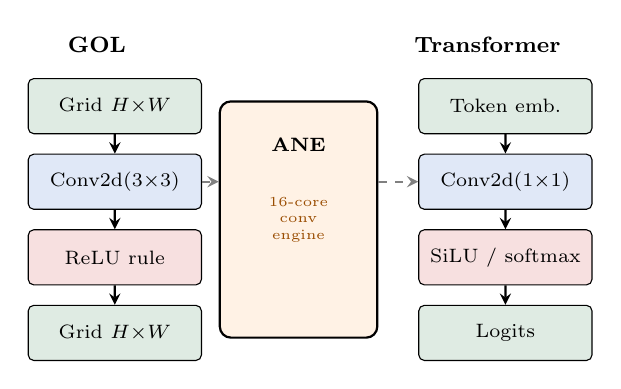
\begin{tikzpicture}[
  scale=0.8,
  box/.style={draw, rounded corners=2pt, minimum height=0.7cm, minimum width=2.2cm, font=\scriptsize, fill=#1!15},
  arr/.style={->, thick, >=stealth}
]
% GOL path
\node[box=alive, anchor=west] (gol_in) at (0, 4.5) {Grid $H{\times}W$};
\node[box=convblue, anchor=west] (gol_conv) at (0, 3.3) {Conv2d(3$\times$3)};
\node[box=relured, anchor=west] (gol_relu) at (0, 2.1) {ReLU rule};
\node[box=alive, anchor=west] (gol_out) at (0, 0.9) {Grid $H{\times}W$};

\draw[arr] (gol_in) -- (gol_conv);
\draw[arr] (gol_conv) -- (gol_relu);
\draw[arr] (gol_relu) -- (gol_out);

\node[font=\footnotesize\bfseries, anchor=south] at (1.1, 5.2) {GOL};

% ANE
\node[draw, thick, rounded corners=4pt, fill=orange!10,
  minimum width=2cm, minimum height=3cm, anchor=center] (ane) at (4.3, 2.7) {};
\node[font=\scriptsize\bfseries, anchor=north] at (4.3, 4.15) {ANE};
\node[font=\tiny, text=orange!60!black, text width=1.6cm, align=center]
  at (4.3, 2.7) {16-core\\conv\\engine};

% Transformer path
\node[box=alive, anchor=west] (tfm_in) at (6.2, 4.5) {Token emb.};
\node[box=convblue, anchor=west] (tfm_conv) at (6.2, 3.3) {Conv2d(1$\times$1)};
\node[box=relured, anchor=west] (tfm_act) at (6.2, 2.1) {SiLU / softmax};
\node[box=alive, anchor=west] (tfm_out) at (6.2, 0.9) {Logits};

\draw[arr] (tfm_in) -- (tfm_conv);
\draw[arr] (tfm_conv) -- (tfm_act);
\draw[arr] (tfm_act) -- (tfm_out);

\node[font=\footnotesize\bfseries, anchor=south] at (7.3, 5.2) {Transformer};

% Connections to ANE
\draw[arr, dashed, gray] (gol_conv.east) -- (ane.west |- gol_conv);
\draw[arr, dashed, gray] (ane.east |- tfm_conv) -- (tfm_conv.west);

\end{tikzpicture}
\caption{Both GOL and the transformer map to convolution on the same
ANE hardware. GOL uses a 3$\times$3 spatial convolution; the
transformer uses 1$\times$1 pointwise convolution. Both are dispatched
to the ANE's 16-core convolution engine.}
\label{fig:unified}
\end{figure}


%% ════════════════════════════════════════════════════════════════════
\section{Optimization Journey}
\label{sec:opt}

The initial implementation produced coherent output at 9~tok/s. A
series of targeted optimizations, many inspired by classic CS texts,
improved this to 90~tok/s---a 10$\times$ improvement.

\subsection{Profiling the Hot Path}

Instrumenting the decode loop revealed three phases per token:

\begin{center}
\footnotesize
\begin{tabular}{lrr}
\toprule
\textbf{Phase} & \textbf{Time (ms)} & \textbf{\%} \\
\midrule
KV cache packing & 0.13 & 1.2\% \\
Model prediction (ANE) & 10.89 & 98.5\% \\
Logit extraction & 0.03 & 0.3\% \\
\midrule
\textbf{Total} & \textbf{11.05} & 100\% \\
\bottomrule
\end{tabular}
\end{center}

The host overhead (pack + extract) is 0.16~ms, reduced from an
initial $\sim$60~ms through the optimizations below.

\subsection{Book-Driven Optimizations}

Four optimization techniques, drawn from classic computer science
texts, collectively eliminated host overhead:

\paragraph{1. Iverson memory layout} (from K.~Iverson, \textit{A
Programming Language}). Pre-allocate KV caches as contiguous
\texttt{[Float16]} arrays in $(n_\text{kv}, \text{maxSeq}, d_h)$
layout, matching the ANE's expected memory order. This eliminated
per-token allocation overhead.

\paragraph{2. Stepanov pre-allocation} (from A.~Stepanov \& P.~McJones,
\textit{Elements of Programming}). Use cursor-based append with
pre-allocated output buffers rather than dynamic array growth. The KV
cache write is a single pointer advance, not a copy.

\paragraph{3. Dragon Book strength reduction} (from A.~Aho et al.,
\textit{Compilers: Principles, Techniques, and Tools}). Replace
high-level \texttt{MLMultiArray} subscript access (which dispatches
through Objective-C) with raw \texttt{Float16} pointer arithmetic and
\texttt{memcpy} for bulk KV cache operations.

\paragraph{4. Brodie data boundaries} (from L.~Brodie,
\textit{Thinking Forth}). Restructure data flow so that the KV cache
format, the model's expected input format, and the host's internal
representation are identical---eliminating all format conversion at
prediction boundaries.

\subsection{Batched GQA}

After host optimization, 98.7\% of time was inside
\texttt{MLModel.prediction()}. Profiling the MIL graph revealed that
672 small per-head matmul operations created scheduling overhead.
Batching all 7 query heads per KV group into single matmuls reduced
MIL operations from 4,569 to 4,399 and improved decode from 78 to
90~tok/s.

\subsection{Hardware Floor Analysis}

The model weights (472~MB, int8) must be loaded from DRAM each token.
At $\sim$100~GB/s unified memory bandwidth, the \emph{theoretical
floor} is:
\begin{equation}
t_\text{floor} = \frac{472 \text{ MB}}{100 \text{ GB/s}} \approx 4.7 \text{ ms}
\end{equation}

Our measured 10.89~ms per token breaks down as:

\begin{center}
\footnotesize
\begin{tabular}{lr}
\toprule
\textbf{Component} & \textbf{Estimated (ms)} \\
\midrule
DRAM weight loading & $\sim$4.7 \\
ANE compute & $\sim$1--2 \\
CoreML dispatch overhead & $\sim$1 \\
Attention (at avg seq$\approx$78) & $\sim$3--4 \\
\midrule
\textbf{Total} & $\sim$10.7 \\
\bottomrule
\end{tabular}
\end{center}

This aligns with measurements, confirming we are near the hardware
limit for this model size on this memory system.


%% ════════════════════════════════════════════════════════════════════
\section{Results}
\label{sec:results}

\subsection{Game of Life}

\begin{table}[t]
\centering
\footnotesize
\begin{tabular}{lrrr}
\toprule
\textbf{Grid} & \textbf{ANE (ms)} & \textbf{CPU (ms)} & \textbf{Speedup} \\
\midrule
$64 \times 64$ & 0.22 & 0.22 & 1.0$\times$ \\
$1024 \times 1024$ & 14.6 & 36.5 & 2.5$\times$ \\
\bottomrule
\end{tabular}
\caption{GOL latency per 32-generation call. ANE advantage grows with
grid size due to spatial parallelism across the 16 cores.}
\label{tab:gol}
\end{table}

At 1024$\times$1024, the ANE achieves $2.3 \times 10^9$
cell-generations/sec with 32 generations pipelined per call.
Verification against CPU reference passes with zero mismatches.

\subsection{Transformer Inference}

\begin{table}[t]
\centering
\footnotesize
\begin{tabular}{llrr}
\toprule
\textbf{Engine} & \textbf{Backend} & \textbf{Prefill} & \textbf{Decode} \\
\midrule
llama.cpp & Metal GPU & 5,978 t/s & 332 t/s \\
GOL-ANE & ANE (conv) & 88 t/s & 90 t/s \\
\bottomrule
\end{tabular}
\caption{Qwen2.5-0.5B-Instruct (Q8\_0) on Apple M3 Pro. GOL-ANE
achieves 90~tok/s decode on a compute unit that llama.cpp does not
use.}
\label{tab:transformer}
\end{table}

The GOL-ANE transformer decode throughput is 3.7$\times$ slower than
llama.cpp on Metal GPU, but operates on an entirely different compute
unit. The ANE path leaves the GPU free for other tasks (rendering,
other models).

\subsection{Optimization Impact}

\begin{figure}[t]
\centering
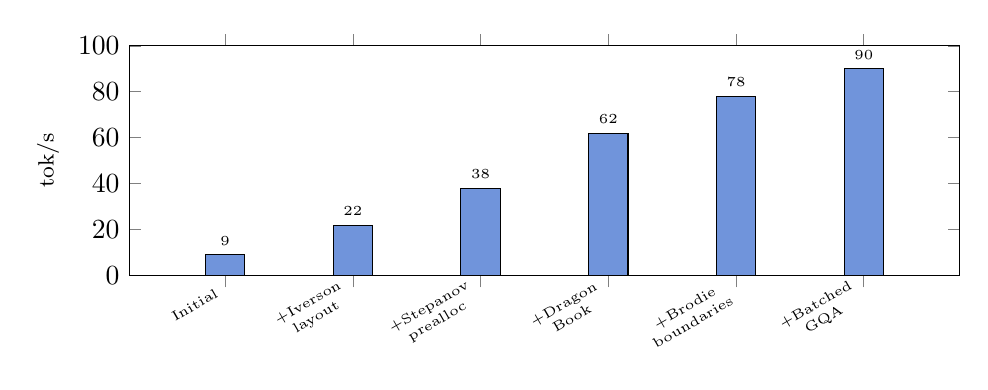
\begin{tikzpicture}
\begin{axis}[
  ybar,
  width=\columnwidth,
  height=4.5cm,
  ylabel={tok/s},
  ylabel style={font=\footnotesize},
  ymin=0, ymax=100,
  xtick=data,
  xticklabels={Initial, +Iverson\\layout, +Stepanov\\prealloc, +Dragon\\Book, +Brodie\\boundaries, +Batched\\GQA},
  xticklabel style={font=\tiny, align=center, rotate=30, anchor=east},
  bar width=0.5cm,
  nodes near coords,
  nodes near coords style={font=\tiny},
  every node near coord/.append style={above},
  enlarge x limits=0.15,
]
\addplot[fill=convblue!70] coordinates {
  (1, 9)
  (2, 22)
  (3, 38)
  (4, 62)
  (5, 78)
  (6, 90)
};
\end{axis}
\end{tikzpicture}
\caption{Cumulative decode throughput improvement from each
optimization. The four book-driven optimizations eliminate host
overhead (9$\to$78 tok/s, 8.7$\times$); batched GQA reduces ANE
scheduling overhead (78$\to$90 tok/s, 1.15$\times$). Total: 10$\times$.}
\label{fig:optbar}
\end{figure}

\subsection{Quantization}

\begin{table}[t]
\centering
\footnotesize
\begin{tabular}{lrrr}
\toprule
\textbf{Quant} & \textbf{Size (MB)} & \textbf{Latency (ms)} & \textbf{tok/s} \\
\midrule
fp16 & 942 & --- & (baseline) \\
int8 & 472 & 6.85 & 146 \\
int4 & 265 & 9.81 & 102 \\
\bottomrule
\end{tabular}
\caption{Quantization benchmark at seq=1 (single-token decode). Int4
is \emph{slower} than int8 due to ANE dequantization overhead.}
\label{tab:quant}
\end{table}


%% ════════════════════════════════════════════════════════════════════
\section{Related Work}
\label{sec:related}

\paragraph{GOL on accelerators.} GPU-based GOL implementations
typically use texture operations or compute shaders~\cite{harris2005}.
HashLife~\cite{gosper1984} achieves exponential speedups for regular
patterns but does not exploit hardware parallelism. Our approach uses
the convolution primitive directly, matching the ANE's native
operation.

\paragraph{LLMs on ANE.} Apple's ml-ane-transformers~\cite{apple2022}
demonstrated channel-last Conv2d layouts for BERT-class models.
Whisper on ANE (via CoreML) uses a similar conv-only approach for the
encoder. Our work extends this to autoregressive generation with KV
caching and demonstrates the GOL connection.

\paragraph{llama.cpp.} The de facto standard for local LLM inference,
using Metal GPU on Apple Silicon~\cite{gerganov2023}. Our work
demonstrates that the ANE---a compute unit llama.cpp does not use---can
achieve meaningful throughput for small models.


%% ════════════════════════════════════════════════════════════════════
\section{Conclusion}

Convolution is enough. Conway's Game of Life and a full transformer
share the same single primitive---convolution---and run on the same
silicon: the Apple Neural Engine's 16-core conv unit. The GOL encoding
is exact (not an approximation), and the transformer produces coherent
text at 90~tok/s.

The optimization journey from 9 to 90~tok/s demonstrates that
classical techniques---memory layout (Iverson), pre-allocation
(Stepanov), strength reduction (Dragon Book), and data boundary
elimination (Brodie)---remain directly applicable to novel hardware
accelerators. The final system operates within $\sim$1~ms of the DRAM
bandwidth floor for its model size.

\paragraph{Future directions.} Pre-allocating output
\texttt{MLMultiArray} buffers to avoid per-call allocation, compiling
multiple models at different sequence lengths, and exploring the ANE's
model-chaining API for zero-copy layer pipelining could further close
the gap to the hardware floor.


%% ════════════════════════════════════════════════════════════════════
\begin{thebibliography}{9}

\bibitem{harris2005}
M.~Harris, \emph{Mapping computational concepts to GPUs},
in GPU Gems 2, Addison-Wesley, 2005.

\bibitem{gosper1984}
R.~W. Gosper, ``Exploiting regularities in large cellular spaces,''
\emph{Physica D}, vol.~10, no.~1--2, pp.~75--80, 1984.

\bibitem{apple2022}
Apple Machine Learning Research, ``Deploying transformers on the Apple
Neural Engine,'' 2022.
\url{https://machinelearning.apple.com/research/neural-engine-transformers}

\bibitem{gerganov2023}
G.~Gerganov, ``llama.cpp: LLM inference in C/C++,'' 2023.
\url{https://github.com/ggerganov/llama.cpp}

\bibitem{iverson1962}
K.~E.~Iverson, \emph{A Programming Language}, John Wiley \& Sons, 1962.

\bibitem{stepanov2009}
A.~A.~Stepanov and P.~McJones, \emph{Elements of Programming},
Addison-Wesley, 2009.

\bibitem{aho2006}
A.~V.~Aho, M.~S.~Lam, R.~Sethi, and J.~D.~Ullman, \emph{Compilers:
Principles, Techniques, and Tools}, 2nd~ed., Addison-Wesley, 2006.

\bibitem{brodie2004}
L.~Brodie, \emph{Thinking Forth}, Punchy Publishing, 2004.

\end{thebibliography}

\end{document}
